\chapter{Background on Convolutional Neural Networks}\label{ch:cnn}
Convolutional neural networks (CNNs) have been one of the most influential innovations in the field of computer vision. Neural networks became popular in 2012 when Alex Krizhevsky used them to win that year's ImageNet competition\cite{alexnet} by dropping the error from 26\% to 15\%. Since then, many companies are using deep learning including Facebook's tagging algorithms, Google for their photo search and Amazon for product recommendations. For the purpose of this thesis CNNs were used for image classification, specifically, images of varying particles created using LArTPC data. 

\section{Image Classification} 
Image classification is the process of inputting an image into the CNN an receiving a probability of classes that best describes what is happening in the image. As humans, image classification is something that is learned at a very young age and is easy to do without much effort. This is also apparent when hand-scanning LArTPC images. After learning what a neutrino event looks like in MicroBooNE, it is relatively easy to recognize simple neutrino events from cosmic ray background as well as highly ionizing particles like protons from minimum ionizing particles like muons. The very detailed images LArTPC detectors output are prime candidates for input images into a CNN. CNNs mimic a human's ability to classify objects by creating an architecture that can learn differences between all the images it's given as well as figure out the unique features that make up each object. CNNs are modeled after the visual cortex. Hubel and Wiesel\cite{hubel} found that there are small regions of neuronal cells in the brain that respond to specific regions of the visual field. They saw that some neurons fired when exposed to vertical edges while others fired when shown horizontal or diagonal edges. They also saw that these neurons were organized in columns. The idea of specific neurons inside of the brain firing to specific characteristics is the basis behind CNNs.

\section{CNN Structure}
When used for image recognition, convolutional neural networks consist of multiple layers that extract different information on small portions of the input image. How many layers is tunable to increase the accuracy. The output of these collections are then tiled so that they overlap to gain a better representation of the original image and allow for translation. The first of these layers is always a convolution layer. To the CNN, an image is an array of pixel values. For a RGB color image with width and height equal to 32x32 the corresponding array is 32x32x3. Filters, also known as neurons, of any size set by the user is then convolved with the receptive field of the image. If the filter is 5x5, the receptive field will by a patch of 5x5 on the input image. The filter is also an array of numbers called weights. The convolution of the filter and image are matrix multiplications of the weights and the pixel values. By stepping the receptive field by 1 unit, for an input image of 32x32x3 and a filter of 5x5x3 you'd get an output array of 28x28x1. This output array is called an activation map or feature map. The use of more filters preserves the spatial dimensions better. The filters can be described as feature identifiers. Examples of features in an image consist of edges, curves, and changes in colors. The first filters in a CNN will primarily be straight line and curve feature identifiers. An example of a curve filter is shown in figure \ref{fig:curvedetector}. When a curve in the same concavity is found in the input image, the corresponding pixel in the output feature map will be activated. Going back to our example of a 32x32 input image and a 5x5 filter, if there were to be a curve in the top left corner of the input image, our output feature map would have a high pixel value in the top left. Therefore, feature maps tell us where a specific feature is located in the original image. Figure \ref{fig:conv1} shows a visualization of filters found in the first layers of many CNN architectures. These filters in the first layer convlove around the image and activate whe nthe specific feature it is looking for is in the receptive field. 
\begin{figure}[htp!]
\centering
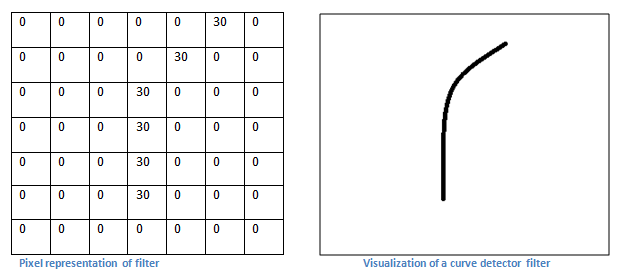
\includegraphics[width=.6\textwidth]{figs/curvedetector.png}
\caption{Pixel representation and visualization of a curve detector filter. As you can see, in the pixel representation, the weights of this filter are greater along a curve we are trying to find in the input image}
\label{fig:curvedetector}
\end{figure} 

\begin{figure}[htp!]
\centering
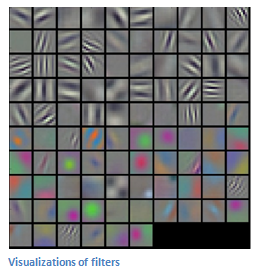
\includegraphics[width=.25\textwidth]{figs/conv1vis.png}
\caption{Visualization of filters found in first layer of a CNN.}
\label{fig:curvedetector}
\end{figure} 

In figure \ref{fig:convolution} you can see how an edge detection filter is used to save only necessary information for recognizing different types of clothes. You can also see by having multiple filters you can get more detail or less detail from an image which can then simplify or complicate the object recognition task. Being able to distinguish between a shirt or a leg garment is as much information you want, having a filter that extracts outline edge or shape information would be all that you need. But if instead you wanted to distinguish between a formal cocktail dress or a summer dress, more information would need to be saved equating to many more filters for one image. Rather than trying to come up with how many filters and what features are important for detection, CNNs do this automatically. CNNs take input parameters, called hyperparameters, for example number of layers, number of filters per layers, number of weights per filter, and uses these to create the output feature maps. The layers build upon each-other, for example if we were creating a CNN for facial recognition the convolutional layers will start learning feature combinations off of the previous layers. The low level features like edges, gradients, and corners of the first layers become high level features like eyes, noses, and hairs. This process is visualized in figure \ref{fig:featuremaps} 

\begin{figure}[t!]
\centering
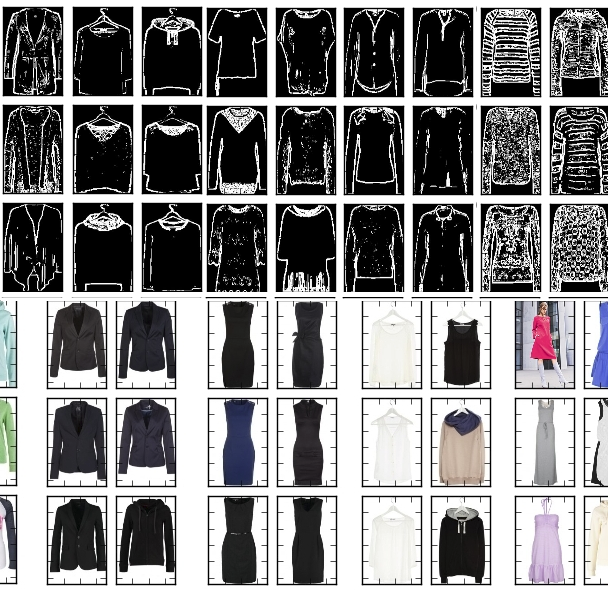
\includegraphics[width=.48\linewidth]{figs/convolution.png}
\caption{Applying a feature mask over a set of fashion items to extract necessary information for auto-encoding. Unnecessary information for example color or brand emblems are not saved. This feature map is an edge detection mask that leaves only shape information which helps to distinguish between different types of clothes.} 
\label{fig:convolution}
\end{figure}

\begin{figure}[h!]
\centering
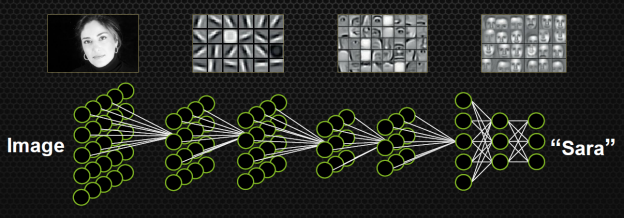
\includegraphics[width=.9\linewidth]{figs/facialDetection.png}
\caption{Pictorial Representation of Convolutional Neural Networks as well as a visual representation on CNN's complexity of layer feature extraction}
\label{fig:featuremaps}
\end{figure}
There are other layers in a CNN architecture that will not be covered in the scope of this thesis but in a general sense, these layers are interspersed between convolution layers to preserve dimensionality and control overfitting of the network. The last layer is called a fully connected layer and it's job is to output an N dimensional vector where N is the number of classes the network has been trained on. Each number in this vector represents the probability that the input image is a certain class. Fully connected layers use the feature maps of the high level features to compute the products between the weights of the previous layer to get the probabilites of each class. These weights are then adjusted throught the training process using backpropagation. 

\subsection{Backpropagation}
A CNN at it's onset has weights that are randomized. The filters themselves don't know how to pull out identifying information per class. For a neural network to learn, it must be trained on a training set that is labeled. Backpropagation has four seperate steps: foward pass, loss function, backward pass and updating weights. In the forward pass, a training image is passed through the whole network. All of our weights at this time are randomly initialized so the output for the first image will have no preference to a specific class. A common loss function is mean squared error (MSE): 
\begin{equation}
E_{total} = \mathlarger{\mathlarger{\sum}}\frac{1}{2}(actual class -predicted class)^2 
\end{equation}

If we assume that the MSE is the loss of our CNN, the goal would be that our predicted label (output of CNN) is the same as our training label. To do this, we need to minimize the loss function. To do this, it is necessary to find out which weights most directly affect the loss of the network i.e $\frac{dL}{dW}$ where L is our loss function and W are the weights of a specific layer. The next step is the backward pass which determines which weights contribute the most to the loss and finds ways to adjust these weights so that the loss decreases. After the derivative is computed, the last step updates the weights in the opposite direction of the gradient. 
\begin{equation}
w=w_i - \eta\frac{dL}{dW}
\\\text{$w$ = Weight}
\\\text{$w_i$ = Initial Weight}
\\\text{$\eta$ = Learning Rate}
\end{equation}

The learning rate is a parameter given to the CNN and it describes the steps the network takes to update the weights. Higher learning rate equals large steps and a lower training time, but a learning rate that is too large can mean the CNN never converges. 

Going through backpropagation consists of one training iteration. Once the network completes a specific number of iterations, another parameter given, and runs over all training images that are split up into batches, the process is considered complete. User input parameters, called hyperparameters, help the network converge to optimal weights for each layer. Batch size, learning rate, and training iteration are just some of the user input hyperparameters that help. Lastly, to check if the network has learned, a different set of labeled images are fed to the CNN iteravely through the training process to see how well it's learning. This process is especially important to make sure the network architecture isn't being affected by overfitting (memorizing training input rather than learning). 

\section{Choosing Hyperparameters}
Convolutional neural networks are a relatively new tools in computer vision. Choosing hyperparameters for your specific dataset is a non-trivial task. Hyperparameters can range from the amount of layers and filters per layer in an CNN architecture to the stride the receptive field of a filter takes, not to mention training hyperparameters such as learning rate and batch size described above. They're ways to optimize these hyperparameters via hyperparameter optimization using Bayesian Optimization \cite{optimization} but as you can imagine, optimizing an CNN architecture from scratch can be very computationally intensive. For the purpose of this thesis, two well known CNN architectures were used, AlexNet \cite{alexnet}, which won the ImageNet Large-Scale Visual Recognition Challenge (ILSVRC) in 2012 and therefore bringing awareness of CNNs, and GoogleNet \cite{googlenet}, which won the ILSVRC in 2014, giving rise to deep networks. Both AlexNet and GoogleNet architectures were used to train on LArTPC images and their low level filter weights. Higher level filter weights were randomly initialized before training so the network can learn high level features of LArTPC image classes. The AlexNet architecture is shown in figure \ref{fig:alexnet} and the GoogleNet architecture is shown in figure \ref{fig:googlenet}

\begin{figure}[htp!]
\centering
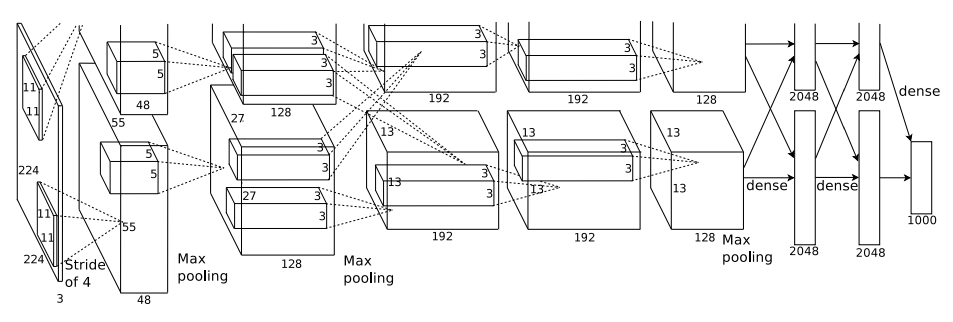
\includegraphics[width=0.9\linewidth]{figs/alexnet.png}
\caption{Pictoral representation of the AlexNet model. The AlexNet model consists of 5 convolution layers and 3 fully connected layers.}
\label{fig:alexnet}
\end{figure}

\begin{figure}[htp!]
\centering
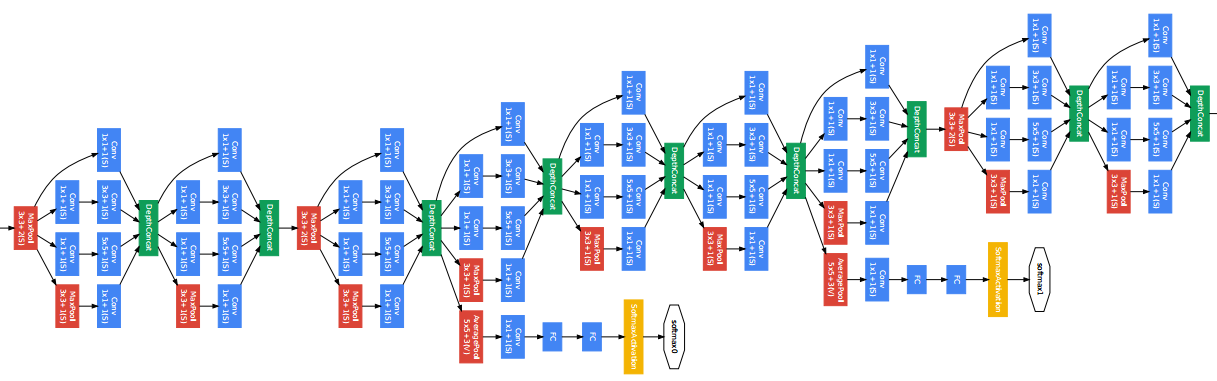
\includegraphics[width=\linewidth]{figs/googlenet.png}
\caption{Pictoral representation of the GoogleNet model. The GoogleNet model consists of 22 layers. The model implements 9 Inception modules which performs covolution and pooling in parallel and strays away from the basis that CNN layers need to be stacked up sequentially. The GoogleNet model also doesn't use fully connected layers, insteat it uses average pooling which greatly reduces the amount of parameters. GoogleNet has 12x fewer parameters than AlexNet. }
\label{fig:googlenet}
\end{figure}
